% answers.tex —— 2011 年·福建卷·文科 · 参考答案与详细解析片段
% 由 tools/generate_projects.py 依来源总账自 2011/2011_数学真题_福建文_试题.md + 2011/2011_数学真题_福建文_解析正文.md + 2011/2011_数学真题_福建文_答案要点.md 生成，勿手改（改源 MD 后重跑）

\begin{answer}
\gksolhead{1}{}

\textbf{题目}：

若集合 $M=\{-1,0,1\}$，$N=\{0,1,2\}$，则 $M\cap N$ 等于\mbox{（　　）}

（A）$\{0,1\}$

（B）$\{-1,0,1\}$

（C）$\{0,1,2\}$

（D）$\{-1,0,1,2\}$

\Needspace{4\baselineskip}
\textbf{解析}
公共元素为 $0,1$，故 $M\cap N=\{0,1\}$。选 A。

\gkanswer{答案：A。}

\end{answer}
\begin{answer}
\gksolhead{2}{}

\textbf{题目}：

$\mathrm i$ 是虚数单位，$1+\mathrm i^3$ 等于\mbox{（　　）}

（A）$\mathrm i$

（B）$-\mathrm i$

（C）$1+\mathrm i$

（D）$1-\mathrm i$

\Needspace{4\baselineskip}
\textbf{解析}
$1+\mathrm i^3=1-\mathrm i$。选 D。

\gkanswer{答案：D。}

\end{answer}
\begin{answer}
\gksolhead{3}{}

\textbf{题目}：

若 $a\in\mathbf R$，则“$a=1$”是“$|a|=1$”的\mbox{（　　）}

（A）充分而不必要条件

（B）必要而不充分条件

（C）充要条件

（D）既不充分也不必要条件

\Needspace{4\baselineskip}
\textbf{解析}
$a=1\Rightarrow|a|=1$；反之 $a=-1$ 也满足，故充分不必要。选 A。

\gkanswer{答案：A。}

\end{answer}
\begin{answer}
\gksolhead{4}{}

\textbf{题目}：

某校选修乒乓球课程的学生中，高一年级有 $30$ 名，高二年级有 $40$ 名。现用分层抽样的方法在这 $70$ 名学生中抽取一个样本，已知在高一年级的学生中抽取了 $6$ 名，则在高二年级的学生中应抽取的人数为\mbox{（　　）}

（A）$6$

（B）$8$

（C）$10$

（D）$12$

\Needspace{4\baselineskip}
\textbf{解析}
抽样比 $\dfrac6{30}=\dfrac15$，高二应抽 $40\times\dfrac15=8$。选 B。

\gkanswer{答案：B。}

\end{answer}
\begin{answer}
\gksolhead{5}{}

\textbf{题目}：

阅读如图所示的程序框图，运行相应的程序，输出的结果是\mbox{（　　）}

（A）$3$

（B）$11$

（C）$38$

（D）$123$
\nopagebreak[4]
\begin{center}% 2011 年福建卷文科第 5 题：程序框图。
% 来源 PDF：普通高考/2011/2011福建文.pdf，SHA-256 e649bdc736a215d4e41e02c6a7945953aca84a87a23e6a903596d61025cdf322。
% 原页：第 1 页第 1 栏中部，书页码 661。
\begin{tikzpicture}[>=stealth, semithick, font=\small]
  \node[draw, rounded corners=0.12cm, minimum width=1.2cm, minimum height=0.5cm] (start) at (0,0) {开始};
  \node[draw, minimum width=1.4cm, minimum height=0.5cm] (a) at (0,-1.1) {$a=1$};
  \node[draw, minimum width=2.4cm, minimum height=0.55cm] (upd) at (0,-2.4) {$a=a^2+2$};
  \node[draw, diamond, aspect=1.7, minimum width=1.5cm, minimum height=0.9cm] (test) at (0,-3.8) {$a<10$};
  \node[draw, trapezium, trapezium left angle=72, trapezium right angle=108,
        minimum width=1.6cm, minimum height=0.55cm] (out) at (0,-5.2) {输出 $a$};
  \node[draw, rounded corners=0.12cm, minimum width=1.2cm, minimum height=0.5cm] (stop) at (0,-6.3) {结束};
  \draw[->] (start)--(a); \draw[->] (a)--(upd); \draw[->] (upd)--(test);
  \draw[->] (test.south)--(out.north) node[midway, right] {否};
  \draw[->] (out)--(stop);
  \draw[->] (test.east) -- ++(1.5,0) |- (upd.east) node[pos=0.25, right] {是};
\end{tikzpicture}
\end{center}
\nopagebreak[4]
\Needspace{4\baselineskip}
\textbf{解析}
$a=1$：$a\leftarrow a^2+2=3<10$；再 $a\leftarrow3^2+2=11\ge10$，输出 $11$。选 B。

\gkanswer{答案：B。}

\end{answer}
\begin{answer}
\gksolhead{6}{}

\textbf{题目}：

若关于 $x$ 的方程 $x^2+mx+1=0$ 有两个不相等的实数根，则实数 $m$ 的取值范围是\mbox{（　　）}

（A）$(-1,1)$

（B）$(-2,2)$

（C）$(-\infty,-2)\cup(2,+\infty)$

（D）$(-\infty,-1)\cup(1,+\infty)$

\Needspace{4\baselineskip}
\textbf{解析}
$\Delta=m^2-4>0$，故 $m<-2$ 或 $m>2$。选 C。

\gkanswer{答案：C。}

\end{answer}
\begin{answer}
\gksolhead{7}{}

\textbf{题目}：

如图，矩形 $ABCD$ 中，点 $E$ 为边 $CD$ 的中点，若在矩形 $ABCD$ 内部随机取一个点 $Q$，则点 $Q$ 取自 $\triangle ABE$ 内部的概率等于\mbox{（　　）}

（A）$\dfrac14$

（B）$\dfrac13$

（C）$\dfrac12$

（D）$\dfrac23$
\nopagebreak[4]
\begin{center}% 2011 年福建卷理科第 4 题：矩形与三角形 ABE。
% 来源 PDF：普通高考/2011/2011福建理.pdf，SHA-256 1a36c388b64669b29d16fe359efb087d96026059df01d26759f8bb5dd48342f1。
% 原页：第 1 页第 1 栏中部，书页码 659。
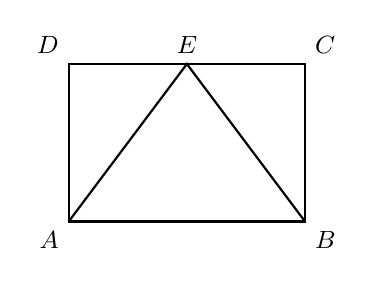
\begin{tikzpicture}[>=stealth, semithick, font=\small, scale=1.0]
  \coordinate (A) at (0,0);
  \coordinate (B) at (3,0);
  \coordinate (C) at (3,2);
  \coordinate (D) at (0,2);
  \coordinate (E) at (1.5,2);
  \draw[thick] (A)--(B)--(C)--(D)--cycle;
  \draw[thick] (A)--(E)--(B);
  \node[below left] at (A) {$A$};
  \node[below right] at (B) {$B$};
  \node[above right] at (C) {$C$};
  \node[above left] at (D) {$D$};
  \node[above] at (E) {$E$};
\end{tikzpicture}
\end{center}
\nopagebreak[4]
\Needspace{4\baselineskip}
\textbf{解析}
$\triangle ABE$ 与矩形同底，高等于矩形宽，面积为矩形一半，概率 $\dfrac12$。选 C。

\gkanswer{答案：C。}

\end{answer}
\begin{answer}
\gksolhead{8}{}

\textbf{题目}：

已知函数 $f(x)=\begin{cases}2^x,&x>0,\\x+1,&x\leqslant0.\end{cases}$ 若 $f(a)+f(1)=0$，则实数 $a$ 的值等于\mbox{（　　）}

（A）$-3$

（B）$-1$

（C）$1$

（D）$3$

\Needspace{4\baselineskip}
\textbf{解析}
$f(1)=2$，故 $f(a)=-2$。若 $a>0$，$2^a>0$ 不可能；故 $a\leqslant0$，$a+1=-2$，$a=-3$。选 A。

\gkanswer{答案：A。}

\end{answer}
\begin{answer}
\gksolhead{9}{}

\textbf{题目}：

若 $\alpha\in\left(0,\dfrac\pi2\right)$，且 $\sin^2\alpha+\cos2\alpha=\dfrac14$，则 $\tan\alpha$ 的值等于\mbox{（　　）}

（A）$\dfrac{\sqrt2}2$

（B）$\dfrac{\sqrt3}3$

（C）$\sqrt2$

（D）$\sqrt3$

\Needspace{4\baselineskip}
\textbf{解析}
\nopagebreak[4]
\[\sin^2\alpha+\cos2\alpha=\sin^2\alpha+1-2\sin^2\alpha=1-\sin^2\alpha=\frac14,\]
故 $\sin^2\alpha=\dfrac34$。$\alpha\in\left(0,\dfrac\pi2\right)$，$\sin\alpha=\dfrac{\sqrt3}2$，$\alpha=\dfrac\pi3$，$\tan\alpha=\sqrt3$。选 D。

\gkanswer{答案：D。}

\end{answer}
\begin{answer}
\gksolhead{10}{}

\textbf{题目}：

若 $a>0$，$b>0$，且函数 $f(x)=4x^3-ax^2-2bx+2$ 在 $x=1$ 处有极值，则 $ab$ 的最大值等于\mbox{（　　）}

（A）$2$

（B）$3$

（C）$6$

（D）$9$

\Needspace{4\baselineskip}
\textbf{解析}
\Needspace{5\baselineskip}
$f'(x)=12x^2-2ax-2b$，$f'(1)=12-2a-2b=0$，故 $a+b=6$。于是
\nopagebreak[4]
\[ab\leqslant\left(\frac{a+b}2\right)^2=9,\]
当 $a=b=3$ 时取等。选 D。

\gkanswer{答案：D。}

\end{answer}
\begin{answer}
\gksolhead{11}{}

\textbf{题目}：

设圆锥曲线 $\Gamma$ 的两个焦点分别为 $F_1$，$F_2$。若曲线 $\Gamma$ 上存在点 $P$ 满足 $|PF_1|:|F_1F_2|:|PF_2|=4:3:2$，则曲线 $\Gamma$ 的离心率等于\mbox{（　　）}

（A）$\dfrac12$ 或 $\dfrac32$

（B）$\dfrac23$ 或 $2$

（C）$\dfrac12$ 或 $2$

（D）$\dfrac23$ 或 $\dfrac32$

\Needspace{4\baselineskip}
\textbf{解析}
三边比 $4:3:2$，$2c$ 对应 $3$。椭圆 $2a=6$，$e=\dfrac12$；双曲线 $2a=2$，$e=\dfrac32$。选 A。

\gkanswer{答案：A。}

\end{answer}
\begin{answer}
\gksolhead{12}{}

\textbf{题目}：

在整数集 $\mathbf Z$ 中，被 $5$ 除所得余数为 $k$ 的所有整数组成一个“类”，记为 $[k]$，即 $[k]=\{5n+k\mid n\in\mathbf Z\}$，$k=0,1,2,3,4$。给出如下四个结论：① $2011\in[1]$；② $-3\in[3]$；③ $\mathbf Z=[0]\cup[1]\cup[2]\cup[3]\cup[4]$；④ “整数 $a$，$b$ 属于同一‘类’”的充要条件是“$a-b\in[0]$”。其中，正确结论的个数是\mbox{（　　）}

（A）$1$

（B）$2$

（C）$3$

（D）$4$

\Needspace{4\baselineskip}
\textbf{解析}
① $2011=5\times402+1$，正确；② $-3=5\times(-1)+2\in[2]$，错误；③ 五个类构成 $\mathbf Z$，正确；④ 同类等价于差被 $5$ 整除，即 $a-b\in[0]$，正确。共 $3$ 个。选 C。

\gkanswer{答案：C。}

\end{answer}
\begin{answer}
\gksolhead{13}{}

\textbf{题目}：

若向量 $\boldsymbol a=(1,1)$，$\boldsymbol b=(-1,2)$，则 $\boldsymbol a\cdot\boldsymbol b$ 等于 $\underline{\qquad}$。

\Needspace{4\baselineskip}
\textbf{解析}
$\boldsymbol a\cdot\boldsymbol b=1\times(-1)+1\times2=1$。

\gkanswer{答案：$1$。}

\end{answer}
\begin{answer}
\gksolhead{14}{}

\textbf{题目}：

若 $\triangle ABC$ 的面积为 $\sqrt3$，$BC=2$，$C=60^\circ$，则边 $AB$ 的长度等于 $\underline{\qquad}$。

\Needspace{4\baselineskip}
\textbf{解析}
\nopagebreak[4]
\[S=\frac12\cdot BC\cdot CA\sin60^\circ=\frac12\cdot2\cdot CA\cdot\frac{\sqrt3}2=\frac{\sqrt3}2CA=\sqrt3,\]
\Needspace{5\baselineskip}
故 $CA=2$。又 $BC=2$，$C=60^\circ$，由余弦定理
\nopagebreak[4]
\[AB^2=4+4-2\cdot2\cdot2\cdot\frac12=4,\]
故 $AB=2$。

\gkanswer{答案：$2$。}

\end{answer}
\begin{answer}
\gksolhead{15}{}

\textbf{题目}：

如图，正方体 $ABCD-A_1B_1C_1D_1$ 中，$AB=2$，点 $E$ 为 $AD$ 的中点，点 $F$ 在 $CD$ 上，若 $EF\parallel$ 平面 $AB_1C$，则线段 $EF$ 的长度等于 $\underline{\qquad}$。
\nopagebreak[4]
\begin{center}% 2011 年福建卷文科第 15 题：正方体与 AD 中点 E、CD 上点 F。
% 来源 PDF：普通高考/2011/2011福建文.pdf，SHA-256 e649bdc736a215d4e41e02c6a7945953aca84a87a23e6a903596d61025cdf322。
% 原页：第 1 页第 2 栏下部，书页码 661。示意。
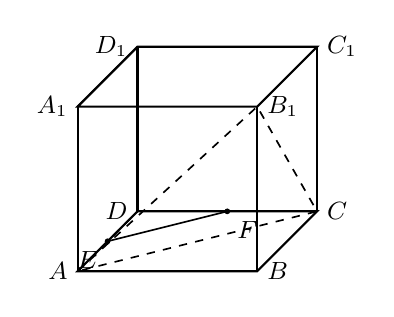
\begin{tikzpicture}[>=stealth, semithick, font=\small, scale=0.95]
  \coordinate (A) at (0,0); \coordinate (B) at (2.4,0);
  \coordinate (C) at (3.2,0.8); \coordinate (D) at (0.8,0.8);
  \coordinate (A1) at (0,2.2); \coordinate (B1) at (2.4,2.2);
  \coordinate (C1) at (3.2,3.0); \coordinate (D1) at (0.8,3.0);
  \coordinate (E) at (0.4,0.4); \coordinate (F) at (2.0,0.8);
  \draw[thick] (A)--(B)--(C)--(D)--cycle;
  \draw[thick] (A1)--(B1)--(C1)--(D1)--cycle;
  \draw[thick] (A)--(A1) (B)--(B1) (C)--(C1) (D)--(D1);
  \draw[dashed] (A)--(D) (D)--(D1) (A1)--(D1);
  \draw (E)--(F);
  \draw[dashed] (A)--(B1)--(C)--(A);
  \fill (E) circle (1.1pt) node[below left] {$E$};
  \fill (F) circle (1.1pt) node[below right] {$F$};
  \node[left] at (A) {$A$}; \node[right] at (B) {$B$};
  \node[right] at (C) {$C$}; \node[left] at (D) {$D$};
  \node[left] at (A1) {$A_1$}; \node[right] at (B1) {$B_1$};
  \node[right] at (C1) {$C_1$}; \node[left] at (D1) {$D_1$};
\end{tikzpicture}
\end{center}
\nopagebreak[4]
\Needspace{4\baselineskip}
\textbf{解析}
\Needspace{5\baselineskip}
设 $A(0,0,0)$，$B(2,0,0)$，$C(2,2,0)$，$D(0,2,0)$，$A_1(0,0,2)$，$B_1(2,0,2)$。平面 $AB_1C$ 的法向量
\nopagebreak[4]
\[\boldsymbol n=\overrightarrow{AB_1}\times\overrightarrow{AC}=(2,0,2)\times(2,2,0)=(-4,4,4)\sim(-1,1,1).\]
\Needspace{5\baselineskip}
$E(0,1,0)$，设 $F(t,2,0)$，则 $\overrightarrow{EF}=(t,1,0)$。由 $EF\parallel$ 平面得 $-t+1=0$，$t=1$。故
\nopagebreak[4]
\[EF=\sqrt{1^2+1^2}=\sqrt2.\]

\gkanswer{答案：$\sqrt2$。}

\end{answer}
\begin{answer}
\gksolhead{16}{}

\textbf{题目}：

商家通常依据“乐观系数准则”确定商品销售价格，即根据商品的最低销售限价 $a$，最高销售限价 $b$（$b>a$）以及实数 $x$（$0<x<1$）确定实际销售价格 $c=a+x(b-a)$。这里，$x$ 被称为乐观系数。经验表明，最佳乐观系数 $x$ 恰好使得 $(c-a)$ 是 $(b-c)$ 和 $(b-a)$ 的等比中项。据此可得，最佳乐观系数 $x$ 的值等于 $\underline{\qquad}$。

\Needspace{4\baselineskip}
\textbf{解析}
\Needspace{5\baselineskip}
$c-a=x(b-a)$，$b-c=(1-x)(b-a)$。由等比中项：
\nopagebreak[4]
\[x^2(b-a)^2=(1-x)(b-a)^2\Longrightarrow x^2=1-x,\]
故 $x=\dfrac{\sqrt5-1}2$（另一根为负，舍）。

\gkanswer{答案：$\dfrac{\sqrt5-1}2$。}

\end{answer}
\begin{answer}
\gksolhead{17}{}

\textbf{题目}：

已知等差数列 $\{a_n\}$ 中，$a_1=1$，$a_3=-3$。

（1） 求数列 $\{a_n\}$ 的通项公式；

（2） 若数列 $\{a_n\}$ 的前 $k$ 项和 $S_k=-35$，求 $k$ 的值。

\Needspace{4\baselineskip}
\textbf{解析}
\gksubpart{(1)}
$a_3=a_1+2d$，$-3=1+2d$，$d=-2$，故 $a_n=1-2(n-1)=3-2n$。

\gksubpart{(2)}
\nopagebreak[4]
\[S_k=\frac{k(1+3-2k)}2=k(2-k)=-35\Longrightarrow k^2-2k-35=0,\]
$k=7$（$k=-5$ 舍）。

\gkanswer{答案（1）：$a_n=3-2n$。}

\gkanswer{答案（2）：$k=7$。}

\end{answer}
\begin{answer}
\gksolhead{18}{}

\textbf{题目}：

如图，直线 $l:y=x+b$ 与抛物线 $C:x^2=4y$ 相切于点 $A$。

（1） 求实数 $b$ 的值；

（2） 求以点 $A$ 为圆心，且与抛物线 $C$ 的准线相切的圆的方程。
\nopagebreak[4]
\begin{center}% 2011 年福建卷文科第 18 题：抛物线 x^2=4y 与切线 l。
% 来源 PDF：普通高考/2011/2011福建文.pdf，SHA-256 e649bdc736a215d4e41e02c6a7945953aca84a87a23e6a903596d61025cdf322。
% 原页：第 1 页第 3 栏中部，书页码 661。
\begin{tikzpicture}[>=stealth, semithick, font=\small, scale=0.9, yscale=1.2]
  \draw[->] (-2.6,0)--(2.6,0) node[right] {$x$};
  \draw[->] (0,-0.8)--(0,3.2) node[above] {$y$};
  \draw[thick, domain=-2.2:2.2, samples=100] plot (\x,{\x*\x/4});
  \draw[thick] (0.5,-1.0)--(2.4,0.4) node[right] {$l$};
  \fill (2,1) circle (1.2pt) node[above right] {$A$};
  \node[below left] at (0,0) {$O$};
  \node at (0.9,2.4) {$C$};
\end{tikzpicture}
\end{center}
\nopagebreak[4]
\Needspace{4\baselineskip}
\textbf{解析}
\gksubpart{(1)}
代入 $y=x+b$：$x^2=4(x+b)$，即 $x^2-4x-4b=0$。相切要求 $\Delta=16+16b=0$，故 $b=-1$。

\gksubpart{(2)}
\Needspace{5\baselineskip}
此时 $x^2-4x+4=0$，$x=2$，$A(2,1)$。准线 $y=-1$，圆心到准线距离 $2$，故半径 $2$，圆为
\nopagebreak[4]
\[(x-2)^2+(y-1)^2=4.\]

\gkanswer{答案（1）：$b=-1$。}

\gkanswer{答案（2）：$(x-2)^2+(y-1)^2=4$。}

\end{answer}
\begin{answer}
\gksolhead{19}{}

\textbf{题目}：

某日用品按行业质量标准分成五个等级，等级系数 $X$ 依次为 $1,2,3,4,5$。现从一批该日用品中随机抽取 $20$ 件，对其等级系数进行统计分析，得到频率分布表如下：

\begin{center}
\begin{tabular}{llllll}
\toprule
$X$ & 1 & 2 & 3 & 4 & 5 \\
\midrule
$f$ & $a$ & 0.2 & 0.45 & $b$ & $c$ \\
\bottomrule
\end{tabular}
\end{center}

（1） 若所抽取的 $20$ 件日用品中，等级系数为 $4$ 的恰有 $3$ 件，等级系数为 $5$ 的恰有 $2$ 件，求 $a$，$b$，$c$ 的值；

（2） 在（1）的条件下，将等级系数为 $4$ 的 $3$ 件日用品记为 $x_1$，$x_2$，$x_3$，等级系数为 $5$ 的 $2$ 件日用品记为 $y_1$，$y_2$，现从 $x_1$，$x_2$，$x_3$，$y_1$，$y_2$ 这 $5$ 件日用品中任取两件（假定每件日用品被取出的可能性相同），写出所有可能的结果，并求这两件日用品的等级系数恰好相等的概率。

\Needspace{4\baselineskip}
\textbf{解析}
\gksubpart{(1)}
\Needspace{5\baselineskip}
由频数 $3,2$ 得 $b=\dfrac3{20}=0.15$，$c=\dfrac2{20}=0.1$，故
\nopagebreak[4]
\[a=1-0.2-0.45-0.15-0.1=0.1.\]

\gksubpart{(2)}
\Needspace{5\baselineskip}
任取两件的所有结果为
\nopagebreak[4]
\[(x_1,x_2),(x_1,x_3),(x_2,x_3),(y_1,y_2),\]
\Needspace{5\baselineskip}
以及 $x_i$ 与 $y_j$ 的 $6$ 个组合，共 $10$ 种。等级系数相等只有前 $4$ 种，故概率
\nopagebreak[4]
\[P=\frac4{10}=\frac25.\]

\gkanswer{答案（1）：$a=0.1$，$b=0.15$，$c=0.1$。}

\gkanswer{答案（2）：所有结果见解析；概率 $\dfrac25$。}

\end{answer}
\begin{answer}
\gksolhead{20}{}

\textbf{题目}：

如图，四棱锥 $P-ABCD$ 中，$PA\perp$ 底面 $ABCD$，$AB\perp AD$，点 $E$ 在线段 $AD$ 上，且 $CE\parallel AB$。

（1） 求证：$CE\perp$ 平面 $PAD$；

（2） 若 $PA=AB=1$，$AD=\sqrt3$，$CD=2$，$\angle CDA=45^\circ$，求四棱锥 $P-ABCD$ 的体积。
\nopagebreak[4]
\begin{center}% 2011 年福建卷文科第 20 题：四棱锥 P-ABCD，PA⊥底面，CE∥AB。
% 来源 PDF：普通高考/2011/2011福建文.pdf，SHA-256 e649bdc736a215d4e41e02c6a7945953aca84a87a23e6a903596d61025cdf322。
% 原页：第 2 页第 1 栏下部，书页码 662。示意。
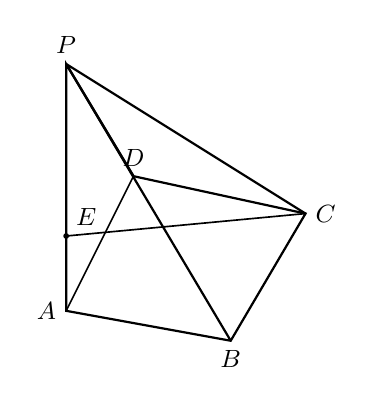
\begin{tikzpicture}[>=stealth, semithick, font=\small, scale=0.95]
  \coordinate (A) at (0,0);
  \coordinate (B) at (2.2,-0.4);
  \coordinate (D) at (0.9,1.8);
  \coordinate (C) at (3.2,1.3);
  \coordinate (E) at (0,1.0);
  \coordinate (P) at (0,3.3);
  \draw[thick] (P)--(A)--(B)--(C)--(D)--cycle;
  \draw[thick] (P)--(B) (P)--(C) (P)--(D);
  \draw (A)--(D);
  \draw (C)--(E);
  \fill (E) circle (1.1pt) node[above right] {$E$};
  \node[left] at (A) {$A$}; \node[below] at (B) {$B$};
  \node[right] at (C) {$C$}; \node[above] at (D) {$D$};
  \node[above] at (P) {$P$};
\end{tikzpicture}
\end{center}
\nopagebreak[4]
\Needspace{4\baselineskip}
\textbf{解析}
\gksubpart{(1)}
$PA\perp$ 底面，故 $PA\perp CE$；又 $CE\parallel AB$，$AB\perp AD$，故 $CE\perp AD$。$PA$、$AD$ 是平面 $PAD$ 内相交直线，故 $CE\perp$ 平面 $PAD$。

\gksubpart{(2)}
取 $A(0,0,0)$，$AB$ 为 $x$ 轴，$AD$ 为 $y$ 轴，$AP$ 为 $z$ 轴。$B(1,0,0)$，$D(0,\sqrt3,0)$，$P(0,0,1)$。由 $CD=2$、$\angle CDA=45^\circ$ 得 $C(\sqrt2,\sqrt3-\sqrt2,0)$。
\Needspace{5\baselineskip}
底面面积
\nopagebreak[4]
\[S_{ABCD}=\frac12\left(\sqrt3-\sqrt2+\sqrt6\right),\]
\Needspace{5\baselineskip}
故
\nopagebreak[4]
\[V=\frac13S_{ABCD}\cdot PA=\frac{\sqrt3-\sqrt2+\sqrt6}6.\]

\gkanswer{答案（1）：证明见解析。}

\gkanswer{答案（2）：$\dfrac{\sqrt3-\sqrt2+\sqrt6}6$。}

\end{answer}
\begin{answer}
\gksolhead{21}{}

\textbf{题目}：

设函数 $f(\theta)=\sqrt3\sin\theta+\cos\theta$，其中角 $\theta$ 的顶点与坐标原点重合，始边与 $x$ 轴非负半轴重合，终边经过点 $P(x,y)$，且 $0\leqslant\theta\leqslant\pi$。

（1） 若点 $P$ 的坐标为 $\left(\dfrac12,\dfrac{\sqrt3}2\right)$，求 $f(\theta)$ 的值；

（2） 若点 $P(x,y)$ 为平面区域 $\Omega:\begin{cases}x+y\geqslant1,\\x\leqslant1,\\y\leqslant1\end{cases}$ 上的一个动点，试确定角 $\theta$ 的取值范围，并求函数 $f(\theta)$ 的最小值和最大值。

\Needspace{4\baselineskip}
\textbf{解析}
\gksubpart{(1)}
\Needspace{5\baselineskip}
$P\left(\dfrac12,\dfrac{\sqrt3}2\right)$ 对应 $\theta=\dfrac\pi3$，
\nopagebreak[4]
\[f(\theta)=2\sin\left(\theta+\frac\pi6\right)=2\sin\frac\pi2=2.\]

\gksubpart{(2)}
\Needspace{5\baselineskip}
区域 $\Omega$ 的顶点为 $(1,0)$，$(1,1)$，$(0,1)$，对应角 $\theta\in\left[0,\dfrac\pi2\right]$。于是
\nopagebreak[4]
\[f(\theta)=2\sin\left(\theta+\frac\pi6\right),\qquad \theta+\frac\pi6\in\left[\frac\pi6,\frac{2\pi}3\right].\]
最小值为 $2\sin\dfrac\pi6=1$（$\theta=0$），最大值为 $2\sin\dfrac\pi2=2$（$\theta=\dfrac\pi3$）。

\gkanswer{答案（1）：$2$。}

\gkanswer{答案（2）：$\theta\in\left[0,\dfrac\pi2\right]$，最小值 $1$，最大值 $2$。}

\end{answer}
\begin{answer}
\gksolhead{22}{}

\textbf{题目}：

已知 $a$，$b$ 为常数，且 $a\neq0$，函数 $f(x)=-ax+b+ax\ln x$，$f(\mathrm e)=2$（$\mathrm e=2.71828\cdots$ 是自然对数的底数）。

（1） 求实数 $b$ 的值；

（2） 求函数 $f(x)$ 的单调区间；

（3） 当 $a=1$ 时，是否同时存在实数 $m$ 和 $M$（$m<M$），使得对每一个 $t\in[m,M]$，直线 $y=t$ 与曲线 $y=f(x)$（$x\in\left[\dfrac1{\mathrm e},\mathrm e\right]$）都有公共点？若存在，求出最小的实数 $m$ 和最大的实数 $M$；若不存在，说明理由。

\Needspace{4\baselineskip}
\textbf{解析}
\gksubpart{(1)}
$f(\mathrm e)=-a\mathrm e+b+a\mathrm e=b=2$。

\gksubpart{(2)}
$f'(x)=-a+a\ln x+a=a\ln x$。故 $a>0$ 时 $0<x<1$ 递减、$x>1$ 递增；$a<0$ 时 $0<x<1$ 递增、$x>1$ 递减。

\gksubpart{(3)}
\Needspace{5\baselineskip}
$a=1$ 时 $f(x)=-x+2+x\ln x$，$f'(x)=\ln x$，在 $\left[\dfrac1{\mathrm e},\mathrm e\right]$ 上最小值 $f(1)=1$。端点
\nopagebreak[4]
\[f\left(\frac1{\mathrm e}\right)=2-\frac2{\mathrm e},\qquad f(\mathrm e)=2.\]
故值域为 $[1,2]$。要每个 $t\in[m,M]$ 都有公共点，需 $[m,M]\subseteq[1,2]$；最小 $m=1$，最大 $M=2$。

\gkanswer{答案（1）：$b=2$。}

\gkanswer{答案（2）：$a>0$ 时减区间 $(0,1)$、增区间 $(1,+\infty)$；$a<0$ 时增区间 $(0,1)$、减区间 $(1,+\infty)$。}

\gkanswer{答案（3）：存在，$m=1$，$M=2$。}

\end{answer}